\documentclass[10pt,twocolumn,letterpaper]{article}

\usepackage{cvpr}
\usepackage{times}
\usepackage{epsfig}
\usepackage{graphicx}
\usepackage{amsmath}
\usepackage{amssymb}

% Include other packages here, before hyperref.

% If you comment hyperref and then uncomment it, you should delete
% egpaper.aux before re-running latex.  (Or just hit 'q' on the first latex
% run, let it finish, and you should be clear).
\usepackage[breaklinks=true,bookmarks=false]{hyperref}

\cvprfinalcopy % *** Uncomment this line for the final submission

\def\cvprPaperID{****} % *** Enter the CVPR Paper ID here
\def\httilde{\mbox{\tt\raisebox{-.5ex}{\symbol{126}}}}

\begin{document}

%%%%%%%%% TITLE
\title{A Generative Model for Brain Tumor Segmentation in Multi-Modal Images}

\author{David Bourque\\
Mcgill University\\
Id: 260670624\\
{\tt\small david.bourque@mail.mcgill.ca}
}

\maketitle
%\thispagestyle{empty}

%%%%%%%%% ABSTRACT
\begin{abstract}
	For this project I chose to attempt to replicate a paper by Bjoern H. Menze, Koen Van Leemput \etal\cite{Menze2010}. In the paper they describe how to build and train a generative model for brain tumor segmentation of multi-modal images. The method is fully automatic, requiring only the images and a probabilistic tissue map, which is assumed to be known. 
\end{abstract}

%%%%%%%%% BODY TEXT
\section{Introduction}

MRI (magnetic resonance imaging) is a common imaging method for the study of brain tumors. Currently, images are  As such there is a need to be able to automatically identify tumors in the scans of a subject. Furthermore modern MRI machines can produce several different types of scans, for example FLAIR, which suppress' cerebrospinal fluid effects on an image, and often images for a patient are available for several different modalities. Standard multi-modal segmentation's (at the time the article was written) find a single tumor region for all modalities, however tumor areas may be delineated differently in each modality. Therefore, delineating tumor areas separately in each modality would be ideal for any further analysis. To that end the authors presented a generative model for multi-modal tumor segmentation that allows for a different segmentation in each modality. For comparison the authors also segmented the images using an EM segmentation similar to \cite{Prastawa}. The authors showed a significant improvement in Dice scores for all modalities they tested (T1, T1 gad, T2 and Flair). For my project I attempted to implement their algorithm and perform segmentation on a data set of multi modal images with glioma's. The paper is outlined as follows: in section 2 I describe the theory behind their algorithm, section 3 describes the data sets I used, section 4 describes my implementation, finally, section 5 I discuss my results (or lack thereof).


%-------------------------------------------------------------------------
\section{Theory}

Descriminitive models attempt to directly predict the desired quantity $p(y|x)$ ($y$ is the presence of tumors in this case), and so, do not consider spatial priors. To do so they generally require a lot of training data. They are also generally limited to the modalities present in the training data. Generative models model the joint probability distribution $p(x,y)$ and use Bayes theorem to try and compute  $p(y|x)$. Using Bayes theorem, in this instance, requires knowing the spatial prior for tumors, which can be difficult to compute. To solve this problem the authors model uses an EM like algorithm to derive the spatial prior (for a particular patient) for tumor tissue. The model also includes a spatial prior on healthy tissues. For their paper, and my project, $K=3$ healthy tissue types were considered, white matter, gray matter and cerebrospinal fluid. See Fig.~\ref{fig:model} for an illustration of the model. Since the algorithm trains and segments simultaneously on a given set of images it generalizes well to any set of modalities. The basic model, while it does consider voxels across channels, does not encode any other spatial information. Although the prior $\pi_k$ does encourage smoothness as neighboring voxels will have similar probabilities. The authors propose an extension to include in $\boldsymbol{\alpha}$ a Markov Random Field spatial prior. They also extend the model to include more tissue classes for tumors, so segment the tumor itself into tissue types, active and necrotic areas etc.. For my project I only implemented the basic model.

\subsection{Model}

The prior on the normal tissue state $K$ is modeled with $\pi_k$, which is a spatial probability map, or atlas, for the 3 tissue types, and is assumed to be known. The atlas defines, for each voxel $i$, a probability of belonging to tissue class $k$:
\begin{equation}p(k_i=k)=\pi_{ki}\end{equation}
The model also uses a latent atlas $\boldsymbol{\alpha}$, which is unknown and derived as part of the algorithm. The latent alpha parametrizes $t$, which is the probability of a tumor at voxel $i$. $t$ takes values $\{0,1\}$ and is modeled as a Bernoulli random variable with probability $\alpha$
\begin{equation}p(t_i = 1)=\alpha_i\end{equation}
The values for $\pi_k$ and $\boldsymbol{\alpha}$ were shared across all channels. 

Observations, $\textbf{y}$, are generated by Gaussian intensity distributions.
An intensity distribution parameter $\boldsymbol{\theta}$ holds parameters $\mu_k^c$ and $v_k^c$ for each of the $C$ channels and $K$ tissue classes, $\mu_{k+1}^c$ and $v_{k+1}^c$ are added for each channel to represent the tumor class. For each voxel $i$ the vector $\textbf{y}_i=[y_i^1,...,y_i^c]$ represents the image observations across all $C$ channels. Similarly the vector $\textbf{t}_i=[t_i^1,...,t_i^c]$ represents the tumor state for all channels at voxel $i$. The authors state the joint probability:
\begin{equation}
p(\textbf{y}_i, \textbf{t}_i, k_i;\boldsymbol{\theta}, \alpha_i) = p(\textbf{y}_i| \textbf{t}_i, k_i;\boldsymbol{\theta})\cdot p(\textbf{t}_i;\alpha_i)\cdot p(k_i)
\end{equation}
Equation 4 in \cite{Menze2010}(See also equations 1,2,3 in \cite{Menze2010}) 

\begin{figure}[t]
	\begin{center}
		%\fbox{\rule{0pt}{2in} \rule{0.9\linewidth}{0pt}}
		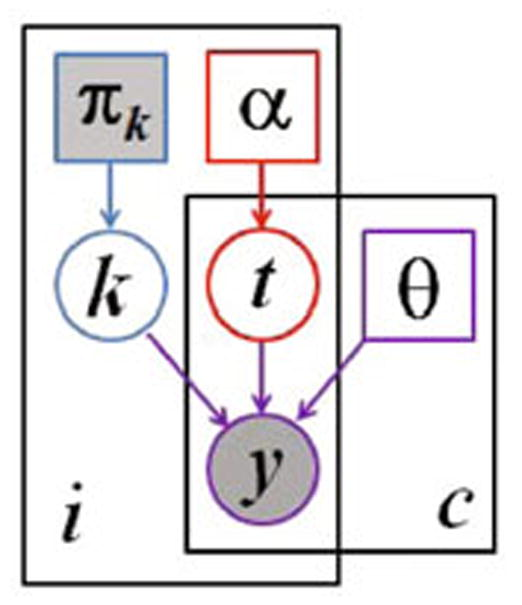
\includegraphics[width=0.5\linewidth]{images/model.jpg}
	\end{center}
	\caption{Graphical model from \cite{Menze2010}. Only shaded values are known. $\pi_k$ is the known prior for healthy tissue. $\textbf{y}$ are image observations}
	\label{fig:model}
\end{figure}

\subsection{Maximum Likelihood and EM}

The intended goal is to find optimal parameters $\{\boldsymbol{\tilde{\theta}},\boldsymbol{\tilde{\alpha}}\}$, that maximize the likelihood of the observations $\boldsymbol{y}_1,...\boldsymbol{y}_N$, where $N$ is the number of voxels. To do so, an EM process is performed, first optimizing $\boldsymbol{\alpha}$, then optimizing $\boldsymbol{\theta}$. Iterations are continued until the maximum likelihood converges. For this they define two functions, one for the probability of any of the $2^C$ possible configurations of $\textbf{t}_i$:
\begin{equation}
q_i(\textbf{t}_i)\triangleq p(\textbf{t}_i|k_i,\textbf{y}_i;\boldsymbol{\theta},\boldsymbol{\alpha})\propto
\sum_{k_i} p(\textbf{y}_i| \textbf{t}_i, k_i;\boldsymbol{\theta})\cdot p(\textbf{t}_i;\alpha_i)\cdot p(k_i)
\end{equation}
Equation 5 from \cite{Menze2010}(See also equations 1,2,3 in \cite{Menze2010})
\\\\
The authors define a similar function $ w_{ik}(\textbf{t}_i)$ for $p(k_i|\textbf{t}_i,\textbf{y}_i;\boldsymbol{\theta},\boldsymbol{\alpha})$, for the posterior probability of $k_i$. These equations are used in the update steps for $\boldsymbol{\alpha}$ and $\boldsymbol{\theta}$ (See unnumbered equations after equation 5 in \cite{Menze2010}).

\subsection{Tumor Segmentation}

A voxel $i$ the in channel $c$ is assigned a value 1 if $p(t_i^c|\textbf{y}_i;\boldsymbol{\tilde{\theta}},\boldsymbol{\tilde{\alpha}})>0.5$ (See equation 6 in \cite{Menze2010})

%-------------------------------------------------------------------------
\section{Data}
In \cite{Menze2010} the authors used an unspecified data set containing 25 sets of patient images. Each set contained T$_{\text{1}}$, T$_{\text{2}}$, FLAIR, and post-Gadolinium T$_{\text{1}}$ images, with tumors manually segmented. For my project I chose to use the BRATS 2013 data set \cite{brats}\cite{virtual_skeleton}. I chose this as it is a publicly available data set, containing real images (some other sets contain synthetic images) with manual segmentation's. Also, Menze, the first author of \cite{Menze2010} is also the first author of \cite{brats}, so they may (although I am guessing) contain some of the same images, although it is not really important. From the data set I chose the 20 sets of images for patients with high grade glioma, with four modalities, T$_{\text{1}}$, T$_{\text{2}}$, T$_{\text{1c}}$, and FLAIR. In each set all images had already been registered to the T$_{\text{1}}$ image, and each set contained a ground truth segmentation. The probabilistic spatial prior used was generated from the probability maps from the MNI-ICBM 152 non-linear atlas, version 2009 \cite{mni1}\cite{mni2}

\section{Experiment}
Before segmentation some preprocessing was necessary. The spatial probability maps were registered onto the T$_{\text{1}}$ image for each set using the advanced normalization tool (ANTs). The registered maps were used to make the spatial prior $\pi_k$. An initial segmentation was also performed, on the T$_{\text{1}}$ images, to initialize variables $\boldsymbol{\theta}$ and $\boldsymbol{\alpha}$.  In \cite{Menze2010}] the authors state they used a freely available implementation of the algorithm in \cite{leemput}, however I was unable to find it. Regardless they segmented the images into 3 healthy classes and an outlier. The outlier was defined as voxels with intensity more than 3 standard deviations away from the mean of any of the 3 tissue classes. For this I again used ANTs, (via Atrapos \cite{atropos}) to segment the images into 3 tissue classes. The mean and standard deviation were calculated for each class, and I further segmented the image by adding the outlier class. Because the segmentation by ANTs was unlabeled, I compared the segmentation's to the spatial prior, which was labeled. The initial segmentation that best matched the spatial prior for tissue $k$ was labeled with class $k$, thus the labels for the atlas $\pi_k$ matched the derived labels for the segmentation. The best match was taken as the class $k$ that had the highest mean probability for all voxels in a particular segmentation. 

Initial $\mu_k^c$ and $v_k^c$ were set based on the segmentation of the healthy tissues, $\mu_{k+1}^c$ and $v_{k+1}^c$ were set with the mean and variance of the outlier class. The latent atlas $\boldsymbol{\alpha}$ was initialized with segmentation of the outlier class, voxels that were part of the outlier class were set to $\alpha_i=0.7$, all other $\alpha_i$ were set to 0.3.

My code was written in python2.7, using jupyter. SimpleITK was used to lead and handle images.

\subsection{results}
Unfortunately, at the time of this writing, I was unable to produce results. I had difficulty with ANTs installation which delayed the project. Mostly, however, it is due to the very large run times for my code. Working with full images, updating $\boldsymbol{\alpha}$ 
\begin{equation}
\alpha_i \leftarrow \sum_{\boldsymbol{t}_i}q_i(\boldsymbol{t}_i)\left( \frac{1}{C}sum_ct_i^c\right)
\end{equation}
Unnumbered equation, below equation 5 in \cite{Menze2010}
\\\\
takes approximately one hour, with the operation vectorized and only those $\alpha_i$ that are not part of the background updated. Updating $\boldsymbol{\theta}$ takes significantly longer,for example the update for $\mu_k^c$ is:
\begin{equation}
\mu_k^c \leftarrow \frac{\sum_i\sum_{\boldsymbol{t}_i}q_i(\boldsymbol{t}_i)w_{ik}(\boldsymbol{t}_i)(1-t_i^c)y_i^c}{\sum_i\sum_{\boldsymbol{t}_i}q_i(\boldsymbol{t}_i)w_{ik}(\boldsymbol{t}_i)(1-t_i^c)}
\end{equation}
Unnumbered equation, under equation 5 in \cite{Menze2010}
\\\\
Similar updates are required for $v_k^c$, $\mu_{k+1}^c$ and $v_{k+1}^c$ for each channel and class, as well as the tumor class for every channel. With $C=4$ and $K=3$ the second step of the EM algorithm requires 16 updates. For the full images I halted the program after it had run for approximately 6 hours and only the first $\mu_1^1$ had been updated. I then shrank the images, with SimpleITK, to $\tfrac{1}{3}$ the size in every dimension. which reduced the total number of voxels from 6 082 560 to 221 328. At this point I was more going for proof of functionality, rather than good results, as such a large decrease in resolution would make any segmentation fairly inaccurate. While running faster the algorithm still took approximately 14 hours to perform one iteration of EM, in \cite{Menze2010} they state it took 10-15 iterations on average to converge, meaning running until convergence would be infeasible, at least considering the due date. Much to my dismay this means I can only claim that my code does not crash. Although I did test many methods individually and am reasonably confident that, given time to run, my code would produce segmentation's. I have since changed the code to operate in 2D, on a single slice from each modality. From manual  inspection of the ground truth I selected a depth in the horizontal plane that contains a large amount of tumor tissue. I then sliced each modality, and the initial segmentation at this same level. The algorithm is currently running, much faster, although i still project time to completion for 10 iterations to be approximately 20 hours. I could again reduce the size of the images, and take a slice, however, considering this project is already overdue I am forced to submit what I have.

\section{Discussion}
The advantages of the authors model are clear, no training set is needed, only the spatial prior, and the model would generalize to any set of MRI images. The authors do not make any mention of run times, and I have no basis for comparison, but it seems to be a very slow algorithm. Granted my computer is dated, and given it never finished, although my program did not crash, the long run time could be due to how I coded the algorithm. It could also be fairly normal, given it segments 4 images simultaneously. However the need to repeatedly sum over the entire image on each iteration, and each sum involving several other nested sums implies a long run time. I am still quite disappointed I was unable to finish any of the segmentation's,and, in hindsight I should have run the program on 2D slices, while there was still time. 

My code is available for review on my github repository at \url{https://github.com/daveguy/ECSEProject.git}
\\\\
Special thanks to Andrew Jenson for his help.



{\small
\bibliographystyle{ieee}
\bibliography{egbib}
Brain tumor image data used in this work were obtained from the NCI-MICCAI 2013 Challenge on Multimodal Brain Tumor Segmentation (http://martinos.org/qtim/miccai2013/index.html) organized by K. Farahani, M. Reyes,B. Menze, E. Gerstner, J. Kirby and J. Kalpathy-Cramer . The challenge database contains fully anonymized images from the following institutions: ETH Zurich, University of Bern, University of Debrecen, and University of Utah and publicly available images from the Cancer Imaging Archive (TCIA).
}

\end{document}
